\section{Highlevel Architecture}
\label{architecture}

\begin{figure}[h]
\begin{center}
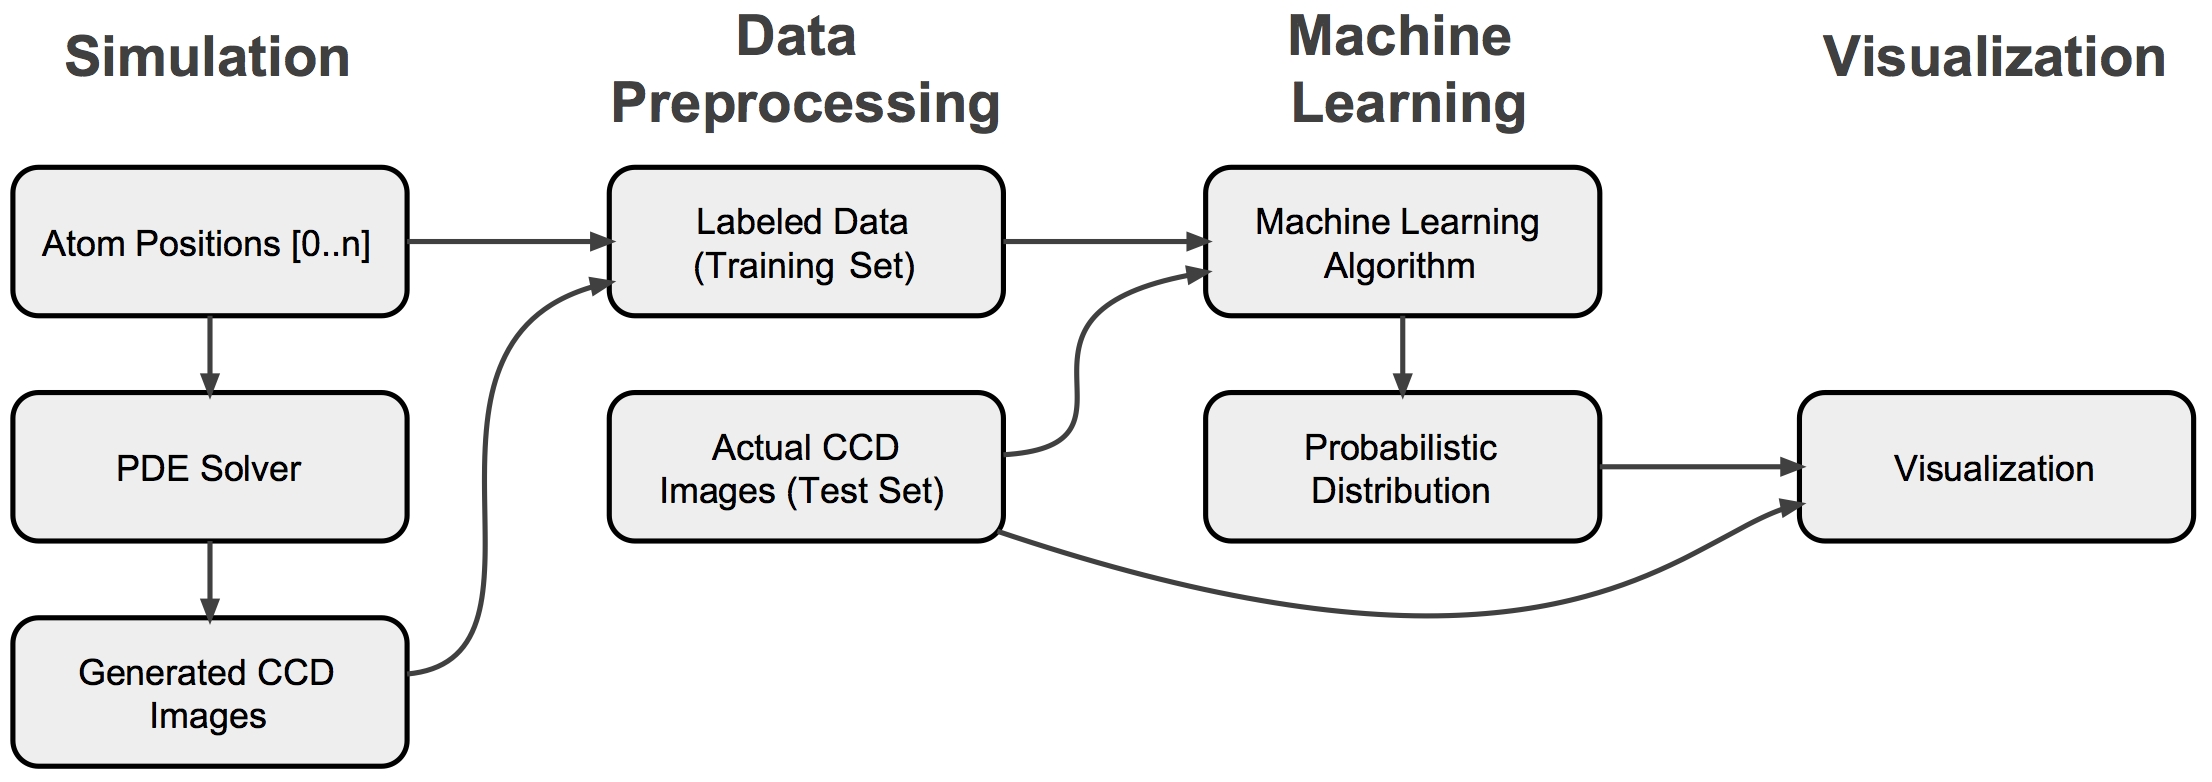
\includegraphics[scale=0.4]{arch.png}
\caption{High Level Data Flow Architecture Diagram}
\label{fig:arch}
\end{center}
\end{figure}

\noindent Figure 1 shows a block level diagram of the project data flow. There are three main components to the solution.
\begin{description}
\item[Simulation] 
\item[Machine Learning] Test multiple machine learning algorithms to find and optimize a strong predictive model.
\item[Visualization]
\end{description}

\subsection{Simulation}
%The core of the simulator is a basic physics simulation. This N-body simulation will track projectiles and vehicles within the world and apply basic Newtonian physics. The simulator will expose the current location of each simulated object at regular intervals as a list of 3D cartesian coordinates and object radii. This stream will be sent using the FOSA format. The simulator will also take in a stream of BDS actions and add projectiles to the simulation as appropriate. The simulator also enforces some sanity rules regarding object motion and provides some basic flight paths for UFOs.

\subsection{Machine Learning}
We will train and test multiple machine learning algorithms on the simulated images by splitting the training data into a training and validation set.  The validation set will be used to determine the best algorithm for this application and then to tune its parameters.  The final classifier will be used to generate probabilistic predictions for the test set of actual CCD images.
 
%AKWDS will take the FOSA stream of object locations and attempt to formulate some tracking of the objects (object A with location $L$ last time step is at location $L'$ this time step). This will be used to help estimate the future location of the object so that targets can be lead correctly for firing. AKWDS will then select a set of object to fire at and set of cannons to fire from and send the needed information via the BDS stream.

\subsection{Visualization}
%Visualization is not a core component of the project deliverable. However AKWDS debugging and demonstration will be very difficult without providing some animation of the system behavior. A visualizer, online or post-hoc, that works from the FOSA stream will be provided to help validate the software.

%\subsection{Data Reduction and Storage}

%We will save the output files onto each node while the simulation is running, and then gather them together on a single head node afterwards. This gives us less of a bottleneck on a single hard drive. During the simulation, the output files will be stored locally on each node, split into files according to the data handled by each node and by the timestep (and perhaps by chunk).

%Addtionally, we can reduce the data size pretty easily I think. It's more work to distribute, and would make our system run faster (maybe even substantially depending on how things pan out). We'll probably be limited by IO, so this actually would be a quick way to improve the speed. Lower priority... 

\subsection{Data Format}

The data will be formatted in the standard Visualization Tool Kit (VTK) format. We will use a regular regtagonal structured grid.